\documentclass[a4paper, 12pt]{article}%тип документа

%%%Библиотеки
	%\usepackage[warn]{mathtext}	
	\usepackage[T2A]{fontenc} % кодировка
	\usepackage[utf8]{inputenc} % кодировка исходного текста
	\usepackage[english,russian]{babel} % локализация и переносы
	\usepackage{caption}
	\usepackage{listings}
	\usepackage{amsmath,amsfonts,amssymb,amsthm,mathtools}
	\usepackage{wasysym}
	\usepackage{graphicx}%Вставка картинок правильная
	\usepackage{float}%"Плавающие" картинки
	\usepackage{wrapfig}%Обтекание фигур (таблиц, картинок и прочего)
	\usepackage{fancyhdr} %загрузим пакет
	\usepackage{lscape}
	\usepackage{xcolor}
	\usepackage[normalem]{ulem}
	\usepackage{hyperref}

%%%Конец библиотек




%%%Настройка ссылок
	\hypersetup
	{
		colorlinks=true,
		linkcolor=blue,
		filecolor=magenta,
		urlcolor=blue
	}
%%%Конец настройки ссылок


%%%Настройка колонтитулы
	\pagestyle{fancy}
	\fancyhead{}
	\fancyhead[L]{Лабораторная работа}
	\fancyhead[R]{Талашкевич Даниил, группа Б01-009}
	\fancyfoot[C]{\thepage}
%%%конец настройки колонтитулы



							\begin{document}
						%%%%Начало документа%%%%


%%%Начало титульника
\begin{titlepage}

	\newpage
	\begin{center}
		\normalsize Московский физико-технический институт \\(госудраственный 			университет)
	\end{center}

	\vspace{6em}

	\begin{center}
		\Large Лабораторная работа по электричеству\\
	\end{center}

	\vspace{1em}

	\begin{center}
		\large \textbf{Измерение магнитного поля Земли [3.1.3]}
	\end{center}

	\vspace{2em}

	\begin{center}
		\large Талашкевич Даниил Александрович\\
		Группа Б01-009
	\end{center}

	\vspace{\fill}

	\begin{center}
	Долгопрудный \\2021
	\end{center}
	
\end{titlepage}
%%%Конец Титульника



%%%Настройка оглавления и нумерации страниц
	\thispagestyle{empty}
	\newpage
	\tableofcontents
	\newpage
	\setcounter{page}{1}
%%%Настройка оглавления и нумерации страниц


					%%%%%%Начало работы с текстом%%%%%%

\textbf{Цель работы:} исследовать свойства постоянных неодимовых магнитов; измерить с их помощью горизонтальную и вертикальную составляющие индукции магнитного поля Земли и магнитное наклонение. \\

\textbf{Используемое оборудование:} неодимовые магниты; тонкая нить для изготовления крутильного маятника; медная проволока; электронные весы; секундомер; измеритель магнитной индукции; штангенциркуль; брусок, линейка и штатив из немагнитных материалов; набор гирь и разновесов.

\section{Теоретическое введение}

Магнитное поле точечного диполя с магнитным моментом $\textbf{m} = \textbf{S}I$ определяется по формуле, аналогичной формуле для поля элементарного электрического диполя:

\begin{equation}
    \textbf{B}_{\text{дип}} = \frac{\mu_0}{4 \pi} \left( \frac{3(\textbf{m} \cdot \textbf{r})\textbf{r}}{r^5} - \frac{\textbf{m}}{r^3}  \right)
\end{equation}

При этом сила, действующая на диполь, равна

\begin{equation}
    \textbf{F} = (\textbf{m} \cdot \triangledown ) \textbf{B}
\end{equation}

А момент силы равен

\begin{equation}
    \textbf{M} = [ \textbf{m} \times \textbf{B}]
\end{equation}

В частном случае, когда моменты двух небольших магнитов направлены вдоль соединяющей их прямой, сила их взаимодействия равна

\begin{equation}
    F = - \frac{6 m_1 m_2}{r^4}
\end{equation}

Если магнитные моменты направлены перпендикулярно соединяющей их прямой, то

\begin{equation}
    F = \frac{3 m_1 m_2}{r^4}
\end{equation}

\section{Экспериментальное оборудование и методика измерений}

\subsection{Определение магнитного момента магнитных шариков}

\subsubsection{Метод 1}

Величину магнитного момента $m$ двух одинаковых шариков можно рассчитать, зная их массу $M$ и определив максимальное расстояние $r_{max}$, на котором они ещё удерживают друг друга в поле тяжести (см. рис.). Из формулы для взаимодействия диполей имеем

\begin{equation}
    m = \sqrt{\frac{Mgr^4_{max}}{6}}
\end{equation}

Таким образом с помощью измеренного магнитного момента шарика можно измерить индукцию магнитного поля

\begin{figure}[h]
    \centering
    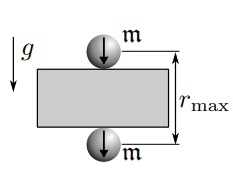
\includegraphics[width = 5 cm]{1.jpg}
    \caption{Измерение магнитных моментов шариков}
    \label{msh1}
\end{figure}

\subsubsection{Метод 2}

Величину магнитного момента шариков можно определить также по силе их сцепления. Она определяется как сила, необходимая для разрыва двух сцепившихся магнитных шариков. Сила сцепления максимальна, если шары соединяются своими противоположными полюсами (магнитные моменты сонаправлены).

Максимальную силу сцепления можно определить по весу магнитной цепочки, которую способен удержать самый верхний магнитный шарик. При этом для расчёта прочности цепочки достаточно учитывать силу взаимодействия верхнего шара с 3–4 ближайшими соседями.

\begin{equation}
    F = \frac{3m^2}{8R^4} \left( 1 + \frac{1}{2^4} + \frac{1}{3^4} + ...\right) = 1,08 \cdot \frac{3m^2}{8R^4}
\end{equation}

\subsection{Измерение горизонтальной составляющей индукции магнитного поля Земли}

Магнитное поле Земли можно измерить по периоду крутильных колебаний «магнитной стрелки» вокруг вертикальной оси.

«Магнитная стрелка» образована сцепленными друг с другом $n$ намагниченными шариками. Для крепления нити в работе используется штатив, изготовленный из немагнитного материала. Магнитные моменты всех шариков направлены в одну сторону вдоль оси «стрелки». При отклонении стрелки на угол $\theta$ от равновесного положения в горизонтальной плоскости возникают крутильные колебания вокруг вертикальной оси, проходящей через середину стрелки.

\begin{figure}[h]
    \centering
    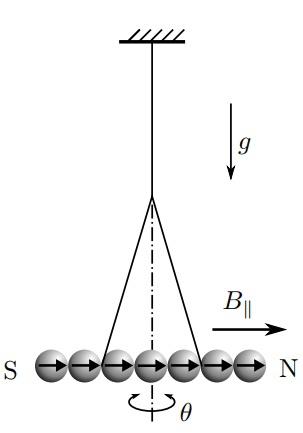
\includegraphics[width = 6 cm]{2.jpg}
    \caption{ Крутильный маятник во внешнем магнитном поле}
    \label{sh1}
\end{figure}

\begin{equation}
    M = -m_n B_{||} \sin{\theta} \Rightarrow J_n \ddot{\theta} + m_n B_{||} \theta = 0 \Rightarrow T = 2 \pi \sqrt{\frac{J_n}{m_n B_{||}}}
\end{equation}

\begin{equation}
    T = 2 \pi \sqrt{\frac{J_n}{m_n B_{||}}} = 2 \pi \sqrt{\frac{n^3 M R^2}{12m_n B_{||}}} \Rightarrow T = 2 \pi \sqrt{\frac{M R^2}{3 m B_{||}}} n
\end{equation}

\subsection{Измерение вертикальной составляющей индукции магнитного поля Земли. Магнитное наклонение}

Для измерения вертикальной составляющей вектора индукции поля Земли используется та же установка, что и для измерения горизонтальной составляющей с тем лишь отличием, что подвешенная магнитная «стрелка» закрепляется на нити в одной точке. В этом случае стрелка, составленная из чётного числа одинаковых шариков и подвешенная за середину, расположится не горизонтально, а под некоторым углом к горизонту.

Это связано с тем, что вектор $\textbf{B}$ индукции магнитного поля Земли не горизонтален, а образует с горизонтом
некоторый угол $\beta$, зависящий от географической широты $\phi$ места, где проводится опыт. Величина угла $\beta$ называется магнитным наклонением.

\begin{figure}[h]
    \centering
    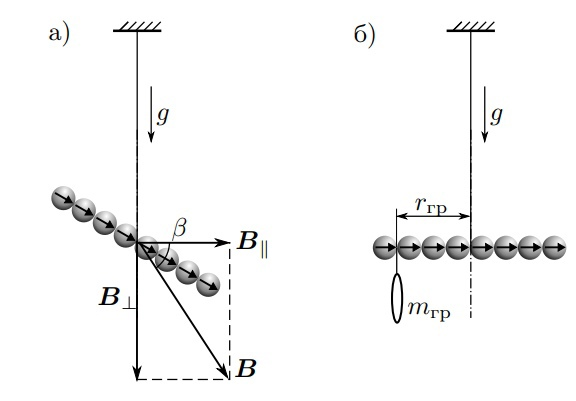
\includegraphics[width = 10 cm]{3.jpg}
    \caption{Измерение вертикальной составляющей поля и магнитного наклонения}
    \label{way3}
\end{figure}

\begin{equation}
    M_n = m B_{\perp} n
\end{equation}

\section{Ход работы}

\subsection{Определение магнитного момента, намагниченности и остаточной магнитной индукции вещества магнитных шариков}

Измерив диаметр и массу шарика, получаем следующие результаты

\[ 	d =	6,4 \pm 0,01 \text{ мм}	  ,\]

\[  	m =	0,841 \pm 0,001	\text{ гр} .\]

С помощью магнетометра измерим индукцию поля $B_p$ на полюсах шарика

\[ B_p = 236,1 \pm 11,8	\text{ мТс} .\]

Проложим между двумя магнитными шариками брусок из немагнитного материала. Увеличивая расстояние между бруском и верхним магнитиком , определим на каком максимальном расстоянии $r_{\max }$ шарики удерживают друг друга в поле тяжести Земли

\[ r_{\max} = 19 \pm 1 \text{мм} .\]

Теперь рассчитаем величину магнитного момента магнитика $m$ и оценим погрешность измерений:

\[ \mathfrak{m}=\sqrt{\frac{m g r_{\max }^{4}}{6}}\ ,\ \]

получаем $\mathfrak{m} = 42,31 \pm \dots$ .

Используя дополнительные шарики, составим цепочку из 20-30 шариков, и с помощью неодимовых магнитов в форме параллелепипедов, подсоединим цепочку к гире и разновесам так, чтобы общая масса системы составила $\sim 250$ г. Добавляя или удаляя шарики, подбераем минимальный вес системы цепочки с гирей, при котором она отрывается от верхнего шарика. Получаем

\[ n = 21	\text{ шарик ,}\]
\[ m = 271,5 \pm 0.021 гр .\]

Рассчитаем силу сцепления двух шаров и по ней определите магнитный момент шарика $\mathfrak{m}$, а так же оцените погрешность результата.

\[ F_{0}=\frac{6 \mathfrak{m}^{2}}{(2 R)^{4}}=\frac{3 \mathfrak{m}^{2}}{8 R^{4}} \quad(\text { ед. } \mathrm{C} \Gamma \mathrm{C}) \]

Тогда минимальный вес цепочки, при которой она оторвётся от верхнего шарика, равен

\[F=F_{0}\left(1+\frac{1}{2^{4}}+\frac{1}{3^{4}}+\frac{1}{4^{4}}+\ldots\right) \approx 1,08 F_{0}\]

Получаем $F = 266070 \text{ дин } \Rightarrow \mathfrak{m} = 71,50 \pm \dots$ .

Оценим полученные значения. Опираться будем на значения, полученные с помощью магнетометра 

\[ B_p = \frac{2}{3} B_r = \frac{2}{3} 4\pi M = \frac{2}{3} 4\pi \frac{\mathfrak{m}}{V} \]

\[ \text{получаем } \mathfrak{m} = \frac{3}{8\pi} B_p V = 38,68 \pm \dots \]

по полученному результату видно, что более точный результат значения магнитных моментов дает метод А. (X про погрешности X)


\subsection{Определение горизонтальной составляющей магнитного поля Земли}

Соберём крутильный маятник из 12 магнитных шариков и подвесим его на немагнитном штативе. Используя $\Lambda$--образный подвес, установим "магнитную стрелку" в горизонтальное положение (юстировка системы).

Возбудим крутильные колебания маятника вокруг вертикальной оси и определим их период. Так же мы легко убедились, что упругость нити на период колебаний можно не учитывать. 

Исследуем зависимость периода $T$ крутильных колебаний "стрелки" от количества магнитных шариков $n$, составляющих "стрелку". Измерения проведём для значений $n = 3, 4, 5, \dots , 12$. Таблица полученных результатов 

\newpage

\begin{table}[!h]
\begin{center}
\begin{tabular}{|c|c|c|c|}
\hline $\mathrm{n}$ & $\mathrm{N}$ & $\mathbf{T}_{\mathrm{N}}$ & $\boldsymbol{T}$ \\
\hline 3 & 20 & 21,20 & 1,06 \\
\hline 4 & 20 & $28,23$ & 1,41 \\
\hline 5 & 20 & 35,25 & 1,76 \\
\hline 6 & 20 & 41,82 & 2,09 \\
\hline 7 & 20 & 48,19 & $2,41$ \\
\hline 8 & 20 & 55,44 & $2,77$ \\
\hline 9 & 20 & 63,02 & $3,15$ \\
\hline 10 & 20 & 68,95 & $3,45$ \\
\hline 11 & 20 & 75,20 & $3,76$ \\
\hline 12 & 20 & 82,00 & 4,10 \\
\hline
\end{tabular}
\caption{время периода колебаний от количества шариков}
\end{center}
\end{table}

Построем график экспериментальной зависимости $T(n)$, а так же убедимся в линейности этой зависимости. По значению углового коэффициента рассчитаем величину горизонтальной составляющей магнитного поля Земли и оценим погрешность полученного результата


\begin{figure}[h]
    \centering
    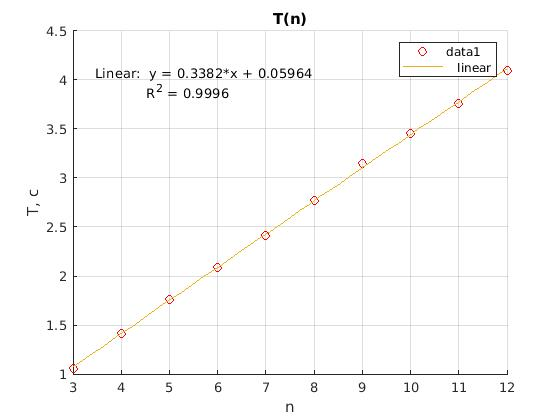
\includegraphics[width = 9 cm]{graph1_s.jpg}
    \caption{график зависимости периода колебаний от числа шариков}
    \label{msh1}
\end{figure}

коэффициент углового наклона $k = 0,3382 \pm = \pi \sqrt{\frac{m R^{2}}{3 \mathfrak{m} B_{\|}}}$. Тогда горизонтальная составляющая магнитного поля $B_{\|} = \dots $ .

\subsection{Определение вертикальной составляющей магнитного поля Земли}

Изготовим магнитную "стрелку" из $n = 10$ шариков и подвесим её за середину с помощью нити на штативе. 

Определим механический момент сил, действующий со стороны магнитного поля Земли на горизонтально расположенную магнитную "стрелку". Для этого, с помощью одного или нескольких кусоч­ков проволоки, уравновесим "стрелку" в горизонтальном положении.

С помощью весов будем определять массу уравновешивающего груза $m_{\text{гр}}$ .

Из условия равновесия рассчитаем механический момент сил $M$, действующих на горизонтальную "стрелку" со стороны поля Земли. Измерения момента сил проведём для чётных значений $n = 4, 6, 8, 10, 12$. Таблица полученных данных

\begin{table}[!h]
\begin{center}
\begin{tabular}{|c|c|c|c|}
\hline $\mathrm{n}$ & $m, \text{гр}$ & $r, \text{см}$ & $\mathrm{M}(\mathrm{n})$ \\
\hline 4 & 0,276 & 0,64 & 173,1072 \\
\hline 6 & 0,152 & 1,28 & 190,6688 \\
\hline 8 & 0,088 & 1,92 & 165,5808 \\
\hline 10 & 0,112 & 2,56 & 280,9856 \\
\hline
\end{tabular}
\caption{зависимость момента сил от кол-ва шариков}
\end{center}
\end{table}

По полученным данным построим график зависимости $\mathrm{M}(\mathrm{n})$


XX

Используя результаты измерений $B_{\perp}$ и $B_{||}$, определим магнитное наклонения $\beta$ и полную величину индукции магнитного поля Земли на широте Долгопрудного.

\[ \beta = \arctan{\frac{B_{\perp}}{B_{||}}} = XX \]

Сравним полученное значение наклонения $\beta$ с расчётным, в предположении, что магнитное поле Земли есть поле однородно намагниченного вдоль оси вращения шара. Оценим также полный магнитный
момент $\mathrm{m}_{\text{З}}$ Земли.

XX

И, наконец, сравним полученные в работе результаты со справочными данными параметров магнитного поля Земли в Московском регионе.





\section{Обработка результатов}

NOTHING

\section{Графики и таблицы}

NOTHING

\section{Вывод}

XX

\section{Литература}

\begin{enumerate}
\item \textbf{Лабораторный практикум по общей физике:} Учебное пособие. В трех томах. Т. 2. Электричество и магнетизм /Гладун А.Д., Александров Д.А., Берулёва Н.С. и др.; Под ред. А.Д. Гладуна - М.: МФТИ, 2007. - 280 с.
\end{enumerate}		
		

\end{document}
